\section{General formation control}
\head{This section will give a short introduction to formation control in general followed by some of the individual assignments which needs to be determined before the process of design can be started.}

The theory of formation control in general is widely applied. It can be applied in assignments regarding control of robots which needs to be placed relative to each other. Depending on the given task of the robots, and which type of robots are in focus, the formation can be utilized in different ways. The robots can also be of various types: Driving vehicles, helicopters, aeroplanes, ships etc. which can both be manned and unmanned. The tasks that these robots needs to fulfill can vary a lot and be both as individuals in a formation or as a whole group. Swarm robots in general got many purposes such as vacuum cleaning robots, who needs to clean a rather large area or flying robots like quadcoptors who can make different kinds of assignments. When quadcoptors work as a combined group they could lift a certain amount of payload to achieve their goal as a group, or they could work individually in a network to do several smaller tasks. An example of how quadcoptors are working together can be examined at \citep{ethswarm}. All these robots are in the terminology called agents. These agents move either individually or in formation. This formation can be rigid or be flexible. If the agents move in rigid formation they will keep their relative positions to each other and does not diverge from the formation. The formation could also be flexible which sometimes proves to be preferable. If the distances between three agents on line are large, and an obstacle needs to be avoided, only one of the agents needs to move from this obstacle if the formation is flexible. This can be seen on figure~\vref{fig:form_avoid_right}.
\begin{figure}[htbp]
	\centering
	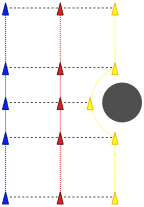
\includegraphics[width=0.5\textwidth]{fig/form_avoid_right}
	\caption{A flexible formation where the right agent avoids an obstacle.}
	\label{fig:form_avoid_right}
\end{figure}

\section{State of the art}
When looking into formation control a lot of different types of control can be taken into control. The main types of formation control are separated into six different types, all under the main topic Multiple Vehicles Coordination Strategies. The overview for this can be found in the survey paper \cite{muv-survey}. The theoretical views on control of \ac{MUV}'s behavior are divided into two classes; centralized and decentralized systems. If the system is centralized this means that all control of the formation is done on one agent, and the others receive information from the core agent. This form of system has the advantage that the core agent can optimize vehicle coordination, accommodate individual agent faults and monitor the accomplishment of the mission. The main disadvantage of this system is that if a fault should occur in the core agent this will affect and facilitate a failure of the whole system. The opposite way of controlling the system would be in a decentralized way. This way of controlling the formation is inspired by the aggregation of birds and fish. This makes each agent able to communicate and share information in between. This means that each agent is given its own part of the complete mission and thus can only complete a part of the mission. The advantage is that faults in a single agent can be overlooked, thus more robust to faults, but can result in a less efficient mission outcome. A decentralized system may be more appropriate to scale up such that more agents can be included and the computational load can, in difference from the centralized system, be split up onto more agents.

The different types of coordination and control algorithms within centralized and decentralized systems include: behavioral-based, virtual structure, leader-follower, graph-based and potential field approaches. Within these structures are the terms Cooperation Control and Formation Control used. Cooperative Control focuses on the global task that the group of agents needs to fulfill, and the Formation Control is the actions performed by each agent which is shared with the other agents in the group. 
\begin{description}[style=nextline]
	\item [Virtual structure]\\
	In a virtual structure is the entire formation treated as a single entity. The behavior coordination for a group of agents in a virtual structure is uncomplicated compared to the coordination of many agents, thus makes this the advantage when doing virtual structure. The disadvantage falls on the centralization due to the structure treated as a single entity. If a failure in this structure happen results in a failure in the entire structure.
	\item [Behavior Based Methods]\\
	The behavioral based model employs several behaviors for each of the agents and the final control used to control the formation is derived from a weighting of the relative importance of each of the behaviors. This could for instance be navigational behaviors to enable a navigation to be the main goal while avoiding hazards and stay in formation.
	\item [Leader-Follower Approaches]\\
	Applying leader-follower methods designates one agent as being the leader and the rest of the agents as followers. The following agents need to position themselves relative to the leader and maintain a desired relative position to the leader. This makes the simplicity to this method, but there is no feedback from the followers to the leader and thus makes that a disadvantage. Within leader-follower methods it is possible to enable changes in the shape of the team. Separation-separation and separation-bearing are two popular leader-follower formation controls, where the followers stay at specified separation and bearing from their designated leader. Within this method it is possible to split the group up into several smaller groups with their individual designated leader.
	\item [Potential Field Approach]\\
	Potential field approaches assigns potentials to agents to make a weighting between them. This weighting could for instance determine the relative distances between the agents. This is usually used when following a virtual leader, such that this process is only made relative to the agents within the structure. This method can make ensure a collision free formation when every agent has been assigned their potential weighting respectively. In this method obstacles can be included and have assigned potentials as well. This will become a avoidance radius from the specific object.
	\item [Graph Theory Approaches]\\
	When applying the graph theory method one assign every agent as a node and assign connections between the nodes. In graph theory this is denoted vertices and edges. The study with graph theory is mainly concentrated of the formation itself and related to changes within the structure. This can be related to the structure within a tree-structure which is used when assigning the formations in graph theory manor. This can be applied as communication analysis for the agents and consensus analysis can be of benefit.
\end{description}

\section{Motivation}


\section{The AAUSHIP project}

\subsection{The mission}
Within the scope of this project the robots will be unmanned ships, \ac{ASV}. The ship's main purpose will be to map the sea bed by using sonars. When one ship need to do this alone, and due to the range of the sonar, the time spend could be improved. The sonar scanning would be done as seen on figure \missingfigure{Billede af enkelt baad som anvender sonar til at scanne havbund}. When only one ship need to map a complete sea bed this process could take up a lot of time dependent on the area that need to be covered. The time spend could be improved to make this mapping more efficient. One way of optimizing the time used is to add more ships to help map the sea bed. To make the process of this as optimal as possible it could be of benefit to implement formation control in the specific assignment. This could be done in several ways, but is mostly thought of in a rigid formation, such that the formation maps the same area of the sea bed the whole time. The idea can be seen on figure \missingfigure{Billede af flere baade som anvender sonar til at scanne havbunden}. The distances between the ships would be determined by how far the sonars could reach the sea bed. There should be some overlap of the maps from each sonar but still as little as possible. The specific formation could be a simple line or it could be more advanced formations. This does not have any relevant impact of how the mappings of the sea bed would be due to the subsequent processing of the collected data from the maps. Different formations of ships can be seen on figure~\vref{fig:diffforms}.
\begin{figure}[htbp]
	\centering
	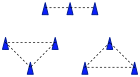
\includegraphics[width=0.5\textwidth]{fig/diffforms}
	\caption{Different formations which the \ac{ASV}s can make.}
	\label{fig:diffforms}
\end{figure}
The formation of the ships may not need to be strictly rigid. Situations could appear where it would be of benefit to change the ship's formation. If the formation need to avoid an obstacle and one or more ships needs to go faster or slower, which leads to a change in the formation, it might be of benefit to regroup the formation which is faster to reach. An example can be seen on figure~\vref{fig:avoid}.
\begin{figure}[htbp]
	\centering
	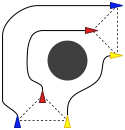
\includegraphics[width=0.5\textwidth]{fig/form_avoid}
	\caption{A formation needs to go around an obstacle where the inner most ship chooses the shortest path and the formation regroups.}
	\label{fig:avoid}
\end{figure}

When doing the formation control it is important to figure out what one
want to achieve, and depending on the strategy and the formation type
some things are to be considered as requirements regarding how the
formation should work. In this discussion lawnmower patterns are considered. In this work two ships are considered for simplicity, but it should be extensible to n-number of ships.

When starting the mission, the ships may start at positions that
is not in the desired formation, it is important that the ships are in
formation when they start tracking the desired track. Therefor some
attention must be given on how to make the ships initialize this
formation. An approach is to make the ships sail individually to the
starting positions with a speed that makes them hit their respectively starting points at
the same time. If one reaches its start point much earlier
than the other it must stop, which is not wanted because it then can
drift out of position again. This basically means that there exists an initialization
phase and a tracking phase. The start heading should of
course align with the path at the start point such that the path following can begin with zero error.

Another issue to be considered is to ensure that no ship at
any point in time reaches a minimum speed that is necessary for the
ship to not drift out of formation. This could be a problem in corners
of the formation if a stiff construction, where the inner most ship
has to move slower, to accommodate the shorter distance on an inner
circle arc.

Faults like blackout on a ship could also be considered in the control
design. I.e. what happens with the formation when one ship faults in a
blackout. Should the rest of the formation stop, should the formation
still follow this drifting ship or should the mission simply terminate
when it is discovered that a ship has blackout.

In the initialization phase it is also relevant to consider how the
ships should avoid each other if they are on the wrong side of each
other.

\begin{figure}[htbp]
	\centering
	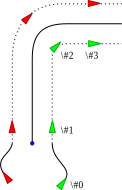
\includegraphics[width=0.6\textwidth]{fig/cornoring}
	\caption{Two ships initializing and following the path offset
		equally on each side, ships are constrained to sailing parallel
		and heading the same as path when projected onto the path. Blue
	dot is start of path. Fully drawn splines is initializing phase.}
	\label{fig:cornoring}
\end{figure}

On figure~\vref{fig:cornoring} is a simple path following performed
with two ships in a stiff formation with an equal distance from the
path. It illustrates four steps. In step \#0 the ships initializes a
random position near the start of the path. At \#1 it is tracking the
path in formation, whilst still in formation. At \#2, the green
(right) ship is in a tight inner curve where it is important to
consider design of the path such that the capabilities of the ship is not
exceeded to stay in formation. At \#3 it is back to straight line path
following in formation. \citep{thorvaldsen}.

\begin{figure}[htbp]
	\centering
	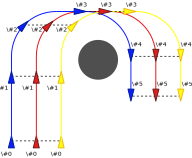
\includegraphics[width=0.6\textwidth]{fig/form_rigid_90}
	\caption{Three ships in formation needs to make a 90\textdegree turn and stays in their relative positions and keeps the rigid formation.}
	\label{fig:form_rigid_90}
\end{figure}

When the ships needs to make a turn about something they can do it in many ways. On figure~\vref{fig:form_rigid_90} the ships keep their formation whilst turning about the object. When they reach the other side and have finished their turn, the ships have kept formation but the outer most ship has now become the inner most ship. The reason to turn like this could be that the inner most ship, the yellow ship, cannot turn as sharp as demanded to stay the inner most ship. Therefore, instead of turning the formation, they stay geometrically rigid.

\begin{figure}[htbp]
	\centering
	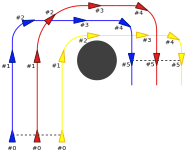
\includegraphics[width=0.6\textwidth]{fig/form_change_90}
	\caption{Three ships in formation needs to make a 90\textdegree turn and changes their relative positions.}
	\label{fig:form_change_90}
\end{figure}

As seen on figure~\vref{fig:form_rigid_90} the ships could have benefit of turning like this. This way of turning could cause trouble in the top of the turn, where the ships eventually will collide due to errors and the relative close distance to each other. This way could be altered a little such that the ships will turn like on figure~\vref{fig:form_change_90}. There the ships adjust their position and velocities to ensure that they will not collide, but they will therefore leave their formation shortly to return back into position again.

\subsubsection{Degree of Actuation}
The degree of actuation is a matter that sets some limitations on how
the path following can be made, and thus the methods available to
control the ships.

AAUSHIP is a ship, which means that is is not fully actuated in the
whole 3D space, but this is not needed since it is moving on a
surface. To be fully actuated it must be able to have controls for
surge, sway and yaw.

\todo{State if it is fully actuated in this sense}

\subsection{Delimitations}
It is chosen to blabla....